\documentclass{rvcepaper}
% s7-common.tex -- macros shared by the Sem 7 CIE papers (\input right after \documentclass{rvcepaper})
% placeholder for text that cannot be read in the scan
\newcommand{\illeg}{\textit{[illegible]}}
\newcommand{\illegc}{{\tiny\textit{[illegible]}}}
% question table with a custom header row: \begin{gtable}[PART -- A]{Sl.\newline No.}{Questions}{M}{BT}{CO}
% the optional title is set as the table's first row so it never strands at a page foot
\newcommand{\gtitlerow}{}
\newenvironment{gtable}[6][]{%
  \def\gtitle{#1}\ifx\gtitle\empty\def\gtitlerow{}\else\def\gtitlerow{\multicolumn{5}{c}{\bfseries\gtitle}\\*[2pt]}\fi
  \begin{longtable}{|C{1.05cm}|p{12.2cm}|C{0.95cm}|C{0.95cm}|C{0.95cm}|}
  \gtitlerow
  \hline \textbf{#2} & \multicolumn{1}{c|}{\textbf{#3}} & \textbf{#4} & \textbf{#5} & \textbf{#6}\\* \hline
  \endfirsthead
  \endhead
}{\end{longtable}}
\newcommand{\twonotes}[2]{{\small Note:}\par\vspace{-1pt}
\hspace*{0.5cm}{\footnotesize 1. \hspace{0.1cm}#1}\par
\hspace*{0.5cm}{\footnotesize 2. \hspace{0.1cm}#2}\par\vspace{3pt}}
\newcommand{\onenote}[1]{{\small Note:}\par\vspace{-1pt}
\hspace*{0.5cm}{\footnotesize 1. \hspace{0.1cm}#1}\par\vspace{3pt}}
% keep the BT/CO caption and the marks-distribution table on the same page
\renewcommand{\btfoot}[2]{\par\vspace{8pt}\noindent\begin{minipage}{\textwidth}\centering
  {\small BT-Blooms Taxonomy, CO-Course Outcomes, M-Marks}\par\vspace{2pt}
  \begin{tabular}{#1}#2\end{tabular}\end{minipage}\par\nopagebreak\vspace{2pt}}
\newcommand{\xfoot}[3]{\par\vspace{8pt}\noindent\begin{minipage}{\textwidth}\centering
  {\small #1}\par\vspace{2pt}\begin{tabular}{#2}#3\end{tabular}\end{minipage}\par\nopagebreak\vspace{2pt}}
\newcommand{\qq}[5]{#1 & #2 & #3 & #4 & #5\\}
\newcommand{\qm}[3]{#1 & #2 & #3\\ \hline}
% other-department header table (Date / Course Code / Sem rows + title row)
\newcommand{\ofour}[7]{\noindent\begingroup\renewcommand{\arraystretch}{1.3}\fontsize{11.5}{13}\selectfont
\begin{tabular}{|C{3.6cm}|C{4.6cm}|C{4.0cm}|C{3.8cm}|}\hline
Date & #1 & Maximum Marks & #2\\\hline
Course Code & #3 & Duration & #4\\\hline
Sem & #5 & \multicolumn{2}{c|}{#6}\\\hline
\multicolumn{4}{|c|}{\bfseries\fontsize{13}{15}\selectfont #7}\\\hline
\end{tabular}\endgroup\par\vspace{6pt}}
\renewcommand{\arraystretch}{1.05}
% the closing stars line stays with the block above it
\renewcommand{\stars}[1]{\par\nopagebreak\vspace{2pt}\nopagebreak\centerline{#1}}
% printed value struck through by hand, with the handwritten correction under it: \corr{60}{34}
\usepackage[normalem]{ulem}
\newcommand{\corr}[2]{\shortstack{\sout{#1}\\#2}}
\usetikzlibrary{decorations.pathmorphing}
% "Academic year" header table without the DEPARTMENT OF block (use inside iempaperB after \paperinfo)
\newcommand{\iemtableB}{%
  \par\vspace{4pt}\noindent\begingroup\renewcommand{\arraystretch}{1.5}\bfseries\fontsize{11.5}{13}\selectfont
  \begin{tabular}{|p{4.2cm}|p{5.0cm}|p{3.7cm}|p{3.6cm}|}\hline
   Date & \getkey{date} & Maximum Marks & \getkey{maxmarks}\\\hline
   Course Code & \getkey{code} & Duration & \getkey{duration}\\\hline
   Sem & \getkey{sem} & \multicolumn{2}{l|}{\getkey{exam}}\\\hline
   \multicolumn{4}{|c|}{\getkey{title}}\\\hline
  \end{tabular}\endgroup\par\vspace{4pt}}
% other-department CIE header: \xdept{Department line}{left1}{mid1}{right1}{left2}{mid2}{right2}{course title cell}{right3}
\newcommand{\xdept}[9]{\par\vspace{2pt}\centerline{\bfseries\fontsize{13.5}{16}\selectfont #1}\par\vspace{4pt}
  \noindent\begingroup\renewcommand{\arraystretch}{1.5}\bfseries\fontsize{11.5}{13}\selectfont
  \begin{tabular}{|p{4.8cm}|C{5.6cm}|p{5.7cm}|}\hline
  #2 & #3 & #4\\\hline #5 & #6 & #7\\\hline \multicolumn{2}{|p{10.8cm}|}{#8} & #9\\\hline
  \end{tabular}\endgroup\par\vspace{8pt}}

\begin{document}

% ---------- 21HS71 Constitution of India and Professional Ethics (Improvement CIE)
\begin{iempaperB}
\paperinfo{ayear={2024-2025 (ODD Sem)},date={17\textsuperscript{th} January 2025},code={21HS71},sem={VII Semester},exam={Improvement CIE},maxmarks={10 + 50},duration={120 Mins},
 title={CONSTITUTION OF INDIA AND PROFESSIONAL ETHICS},shownote=0}
\iemheadB
\onenote{Answer all the Questions.}
\begin{gtable}[PART -- A]{Sl.\newline No.}{Questions}{M}{BT}{CO}
\q{1}{\blank[2.4cm] is termination by the employer of the service of a worker for any reason whatsoever, otherwise than as a punishment inflicted by way of disciplinary action.}{01}{2}{2}
\q{2}{The \blank[2.4cm] Act provides certain benefits to employees in case of sickness, maternity and employment injury, related matters.}{01}{1}{2}
\q{3}{The working hours of an adolescent worker shall be regulated in accordance with the provisions of the \blank[2.4cm] Act.}{01}{2}{2}
\q{4}{List any two Roles Played By the CSR Committee}{01}{2}{2}
\q{5}{List any two objectives of Industrial policy in India}{02}{2}{2}
\q{6}{What is child labor?}{02}{1}{3}
\q{7}{What is Fault Tree Analysis Approach?}{02}{3}{1}
\end{gtable}
\begin{gtable}[PART -- B]{Sl.\newline No.}{Questions}{M}{BT}{CO}
\q{1.}{Define Corporate Social Responsibility? Explain the role of and responsibilities of CSR in society with two cases.}{10}{2}{4}
\q{2.}{Discuss the Guidelines stipulated for Universities and colleges to curb the menace of ragging.}{10}{1}{3}
\q{3}{Explain the prohibition and prevention of sexual harassment of women employee in working place with decided case study.}{10}{3}{3}
\q{4}{Highlight the thrust areas of Government in framing labour laws and list various labour legislation laws enacted by Central Government.}{10}{2}{2}
\q{5}{Define Industrial dispute. Explain the mechanism for resolving Industrial disputes under the Industrial dispute Act 1947.}{10}{2}{4}
\end{gtable}
\btfoot{|l|l|l|*{5}{C{0.8cm}|}*{6}{C{0.8cm}|}}{\hline
\multirow{3}{*}{Marks Distribution} & \multicolumn{2}{c|}{Particulars} & CO1 & CO2 & CO3 & CO4 & CO5 & L1 & L2 & L3 & L4 & L5 & L6\\\cline{2-14}
 & \multirow{2}{*}{\shortstack{Max\\Marks}} & Quiz & -- & & -- & -- & -- & -- & 10 & -- & -- & -- & --\\\cline{3-14}
 & & Test & -- & 10 & 20 & 20 & -- & 10 & 30 & 10 & - & - & --\\\hline}
\end{iempaperB}

% ---------- 21IM72 Product Design & Development (Improvement CIE)
\begin{iempaperB}
\paperinfo{ayear={2024-2025 (ODD Sem)},date={17\textsuperscript{th} February 2025},code={21IM72},sem={VII Semester},exam={Improvement CIE},maxmarks={10 + 50},duration={120 Mins},
 title={PRODUCT DESIGN \& DEVELOPMENT},shownote=0}
\iemheadB
{\small Note:}\par\vspace{-1pt}
\hspace*{0.5cm}{\footnotesize 1. \hspace{0.1cm}Answer all the Questions.}\par
\hspace*{0.5cm}{\footnotesize 2. \hspace{0.1cm}Avoid verbose answers and answer specifically and to the point.}\par
\hspace*{0.5cm}{\footnotesize 3. \hspace{0.1cm}Sketches must be provided in Part B answers as appropriate.}\par
\hspace*{0.5cm}{\footnotesize 4. \hspace{0.1cm}Engineering specifications and Qualitative and/or Quantitative metrics must be mentioned in Part B answers appropriately.}\par\vspace{3pt}
\begin{gtable}[PART -- A]{Sl.\newline No.}{Questions}{M}{BT}{CO}
\q{1}{What is the role of Monte Carlo simulation in risk analysis for product development projects?}{01}{L$_2$}{CO4}
\q{2}{How does Design Structure Matrix (DSM) help in managing dependencies in iterative product design projects?}{01}{L$_2$}{CO4}
\q{3}{Name one key risk associated with product design and development projects.}{01}{L$_2$}{CO4}
\q{4}{What is meant by ``design parallelism'' in Concurrent Engineering?}{01}{L$_2$}{CO3}
\q{5}{What impact does Concurrent Engineering have on reducing design iterations and rework?}{01}{L$_2$}{CO3}
\q{6}{How does Industrial Design differ from Engineering Design?}{01}{L$_2$}{CO3}
\q{7}{Why is Biomechanics important in Ergonomics for product design?}{01}{L$_2$}{CO3}
\q{8}{How do designers use eye-tracking technology in Ergonomic studies?}{01}{L$_2$}{CO4}
\q{9}{How does the Fitts' Law apply to Ergonomic design in interactive products?}{01}{L$_2$}{CO4}
\q{10}{What is the importance of Grip Design in handheld product development?}{01}{L$_2$}{CO4}
\end{gtable}
\begin{gtable}[PART -- B]{Sl.\newline No.}{Questions}{M}{BT}{CO}
\q{1.}{How does cross-functional team collaboration improve the efficiency of product development projects? Provide real world industry based examples.}{10}{L$_4$}{CO3}
\q{2.}{Explain how simultaneous product and process development helps improve efficiency in Concurrent Engineering. Discuss with two case examples.}{10}{L$_3$}{CO3}
\q{3.}{Explain how 3D Printing and Additive Manufacturing are transforming Industrial Design. Discuss advantages and limitations, Discuss using examples.}{10}{L$_3$}{CO4}
\q{4.}{Discuss how sports equipment design (e.g., running shoes, bicycles) integrates Industrial Design and Ergonomics for better performance. Specific product features covering performance, ergonomics and industrial design must be illustrated with appropriate sketches.}{10}{L$_4$}{CO4}
\q{5.}{Explain the role of sustainability in Industrial Design. How can sustainable design principles be integrated into product development? Give two case examples with supporting illustrative sketches.}{10}{L$_4$}{CO4}
\end{gtable}
\btfoot{|l|l|l|*{5}{C{0.8cm}|}*{6}{C{0.8cm}|}}{\hline
\multirow{3}{*}{Marks Distribution} & \multicolumn{2}{c|}{Particulars} & CO1 & CO2 & CO3 & CO4 & CO5 & L1 & L2 & L3 & L4 & L5 & L6\\\cline{2-14}
 & \multicolumn{2}{c|}{} & \multicolumn{11}{c|}{\illeg\ (cut off in the scan)}\\\hline}
\end{iempaperB}

% ---------- 21IM78 Innovation and Entrepreneurship (Improvement CIE)
\begin{iempaperB}
\paperinfo{ayear={2024-2025 (ODD Sem)},date={19\textsuperscript{th} February 2025},code={21IM78},sem={VII Semester},exam={Improvement CIE},maxmarks={05 + 25},duration={60 Mins},
 title={INNOVATION AND ENTREPRENEURSHIP},shownote=0}
\iemheadB
{\small Note:}\par\vspace{-1pt}
\hspace*{0.5cm}{\footnotesize 1. \hspace{0.1cm}Answer all the Questions.}\par
\hspace*{0.5cm}{\footnotesize 2. \hspace{0.1cm}Use suitable sketches and tabular column wherever necessary.}\par
\hspace*{0.5cm}{\footnotesize 3. \hspace{0.1cm}Observe the marks split-up and answer accordingly.}\par\vspace{3pt}
\begin{gtable}[PART -- A]{Sl.\newline No.}{Questions}{M}{BT}{CO}
\q{1}{Comment on the importance of Maximization with regard to pricing strategies.}{01}{L1}{CO1}
\q{2}{Provide two examples business that you can start now by using your existing skills and generate revenue with bootstrapping.}{01}{L4}{CO2}
\q{3}{Identify any two secondary revenue streams.}{02}{L1}{CO2}
\q{4}{Comment on how startups have used ``Content Marketing'' effectively to bring awareness to their offerings with an example.}{01}{L3}{CO3}
\end{gtable}
\begin{gtable}[PART -- B]{Sl.\newline No.}{Questions}{M}{BT}{CO}
\q{1.}{Write short notes on
\begin{romi}\item Segmentation and Targeting\item Importance of Early adopters\end{romi}}{5}{2}{2}
\q{2.}{Suggest a solution demo for any two of the following companies:
\begin{romi}\item A company building houses on wheels\item A company manufacturing grocery bags that dissolve in water\item A company that has made an app for visually challenged people\item A company that rents furniture\end{romi}}{2.5 *2 = 5}{3}{3}
\q{3.}{Explain how Minimum Viable Product helps in Potential Risk reduction.}{5}{3}{4}
\q{4.}{Taking an example of Cirque De Sole or any other example of your choice, Illustrate the 4-action framework by plotting strategy canvas to take advantage of uncontested market.}{5}{3}{4}
\q{5.}{What are the key benefits of using social media marketing for brand engagement?}{5}{2}{4}
\end{gtable}
\btfoot{|l|l|l|*{5}{C{0.8cm}|}*{6}{C{0.8cm}|}}{\hline
\multirow{3}{*}{\shortstack{Marks\\Distribution}} & \multicolumn{2}{c|}{Particulars} & CO1 & CO2 & CO3 & CO4 & CO5 & L1 & L2 & L3 & L4 & L5 & L6\\\cline{2-14}
 & \multirow{2}{*}{\shortstack{Max\\Marks}} & Quiz & 01 & 03 & 01 & -- & -- & 01 & 01 & 01 & 02 & -- & --\\\cline{3-14}
 & & Test & -- & 05 & 12 & 08 & -- & -- & 05 & 05 & 05 & 10 & --\\\hline}
\stars{*****}
\end{iempaperB}

% ---------- 21IM73G1 Data Mining and Predictive Analytics (Elective, Improvement CIE)
\begin{iempaperB}
\paperinfo{ayear={2024-2025 (ODD Sem)},date={18\textsuperscript{th} February 2025},code={21IM73G1},sem={VII Semester},exam={Improvement CIE},maxmarks={10 + 50},duration={120 Mins},
 title={DATA MINING AND \ PREDICTIVE ANALYTICS (Elective)},shownote=0}
\iemheadB
\twonotes{Answer all the Questions.}{Avoid verbose answers and answer specifically and to the point.}
\begin{gtable}[PART -- A]{Sl.\newline No.}{Questions}{M}{BT}{CO}
\q{1}{Why are distance metrics important in clustering algorithms?}{01}{L$_2$}{CO1}
\q{2}{What is a dendrogram, and how is it used in hierarchical clustering?}{01}{L$_2$}{CO1}
\q{3}{What is the significance of ``random'' in Random Forest?}{01}{L$_2$}{CO1}
\q{4}{Can Random Forest be used for both classification and regression tasks?}{01}{L$_2$}{CO1}
\q{5}{How does Gradient Boosting differ from Random Forest?}{01}{L$_2$}{CO1}
\q{6}{What is the role of the learning rate in Gradient Boosting?}{01}{L$_2$}{CO2}
\q{7}{How does anomaly detection differ from outlier detection?}{01}{L$_3$}{CO2}
\q{8}{Describe one advantage of using unsupervised learning for anomaly detection.}{01}{L$_3$}{CO2}
\q{9}{Name one advantage of using ensemble methods over a single predictive model.}{01}{L$_1$}{CO2}
\q{10}{What does the term ``bagging'' refer to in ensemble techniques}{01}{L$_1$}{CO2}
\end{gtable}
\begin{gtable}[PART -- B]{Sl.\newline No.}{Questions}{M}{BT}{CO}
\q{1.}{Consider five data points in 1D:\newline
A=1 A = 1, B=3 B = 3, C=4 C = 4, D=8 D = 8, and E=10 E = 10.
\begin{romi}\item Compute the pairwise Euclidean distances between these points.\item Using single linkage, perform agglomerative clustering until you have two clusters. List the clusters at each step.\end{romi}
\textit{Hint:} In single linkage, the distance between two clusters is the minimum distance between any pair of points in the two clusters.}{10}{L$_2$}{CO1}
\q{2.}{You are building a decision tree for a binary classification problem where you have the following data at a node:
\qtabc{|l|l|}{\hline Class & Count\\\hline 0 & 30\\\hline 1 & 70\\\hline}
\begin{romi}\item Calculate the Gini impurity for the current node.\item Suppose the dataset is split into two groups, one with 10 class 0 and 30 class 1, and the other with 20 class 0 and 40 class 1. Calculate the Gini impurity for each of the two splits and compute the weighted average Gini impurity for the entire split.\end{romi}}{10}{L$_2$}{CO2}
\q{3.}{Suppose you have a binary classification problem with the following dataset:
\qtabc{|C{1.6cm}|C{1.6cm}|C{1.6cm}|}{\hline x1 & x2 & y\\\hline 2 & 3 & 0\\\hline 1 & 4 & 1\\\hline 3 & 2 & 0\\\hline 4 & 3 & 1\\\hline}
You decide to use Gradient Boosting Classifier with decision stumps as base learners. For simplicity, let's use a learning rate of $\eta$=0.1 and fit one shallow tree (stump) at each boosting iteration.}{05}{L$_3$}{CO2}
\q{4.}{Describe the concept of Text Mining and how it is applied in extracting meaningful information from large volumes of unstructured text data. Provide an example of a text mining application.}{15}{\illegc}{\illegc}
\q{5.}{You are given a dataset containing the transaction details of a credit card company. The dataset includes the following features: transaction amount, transaction time, transaction location, and the customer's previous transaction history. Define what anomaly detection is and explain its importance in the context of credit card fraud detection. Give one more example based on the above description.}{10}{\illegc}{\illegc}
\end{gtable}
\btfoot{|l|l|l|*{5}{C{0.8cm}|}*{6}{C{0.8cm}|}}{\hline
\multirow{3}{*}{Marks Distribution} & \multicolumn{2}{c|}{Particulars} & CO1 & CO2 & CO3 & CO4 & CO5 & L1 & L2 & L3 & L4 & L5 & L6\\\cline{2-14}
 & \multirow{2}{*}{\shortstack{Max\\Marks}} & Quiz & 05 & 05 & -- & -- & -- & 02 & 06 & 02 & -- & \illegc & \illegc\\\cline{3-14}
 & & Test & 10 & 40 & -- & -- & -- & -- & 35 & 05 & 10 & \illegc & \illegc\\\hline}
\stars{***********}
\end{iempaperB}

% ---------- 21IM73GC Virtual Commerce (Department Elective, Improvement CIE)
\begin{iempaperB}
\paperinfo{ayear={2024-2025 (ODD Sem)},date={18\textsuperscript{th} February 2025},code={21IM73GC},sem={VII},exam={Improvement \ CIE},maxmarks={10 + 50},duration={120 Mins},
 title={VIRTUAL COMMERCE (Department Elective)},shownote=0}
\iemheadB
{\small Note: Answer all the Questions.}\par\vspace{3pt}
\begin{gtable}[PART -- A]{Sl.\newline No.}{Questions}{M}{BT}{CO}
\q{1}{What are the key limitations of the current internet infrastructure in meeting the increasing demands of modern society?}{02}{L2}{CO1}
\q{2}{How can decline costs of IoT devices be applied to maintain reliability and minimize error rates in a large-scale deployment?}{02}{L2}{CO2}
\q{3}{What is the role of internet access drones in improving internet connectivity, particularly in remote areas?}{02}{L1}{CO3}
\q{4}{What is \ the impact of fiber optics in the First Mile on the overall performance of internet services, considering bandwidth and scalability.}{02}{L2}{CO2}
\q{5}{Compare the strengths and weaknesses of mobile internet access vs. telephone-based internet in the Last Mile, focusing on reliability.}{02}{L2}{CO3}
\end{gtable}
\begin{gtable}[PART -- B]{Sl.\newline No.}{Questions}{M}{BT}{CO}
\q{1.}{Analyze the limitations of the current internet infrastructure in handling the increasing demands of modern society. Evaluate how the introduction of Internet2\textregistered\ could address these limitations. Furthermore, assess the impact of government regulation and surveillance on the internet, considering both societal benefits and privacy concerns. How do these regulations influence the development of future internet technologies, and what balance should be struck between security and privacy?}{10}{L4}{CO4}
\q{2.}{Analyze the challenges and advantages of deploying fiber optic technology in the First Mile for handling the bandwidth explosion. How does it impact the scalability and reliability of internet infrastructure? In the context of the Last Mile, compare and evaluate mobile internet access versus telephone-based internet access in terms of speed, accessibility, and reliability. How do these two access technologies influence the overall performance and equity of global internet connectivity?}{10}{L4}{CO4}
\q{3.}{imagine you are tasked with improving internet latency for a global online gaming platform. Apply your knowledge of future internet latency solutions (such as edge computing, 5G, or satellite networks) to propose a set of strategies that could reduce latency and improve the user experience. How would you prioritize and implement these strategies in a high-traffic gaming environment?}{10}{L3}{CO3}
\q{4.}{Given the increasing deployment of IoT devices in smart homes and industrial settings, apply your knowledge of guaranteed service levels and lower error rates to design an IoT-based solution that ensures optimal performance and reliability. How would you implement a system that balances low error rates with maintaining the cost-effectiveness of the solution, considering the declining costs of IoT devices?}{10}{L3}{CO1}
\q{5.}{How has Social Commerce evolved over time? What are its advantages and disadvantages?}{10}{L2}{CO2}
\end{gtable}
\btfoot{|l|l|l|*{5}{C{0.8cm}|}*{6}{C{0.8cm}|}}{\hline
\multirow{3}{*}{Marks Distribution} & \multicolumn{2}{c|}{Particulars} & CO1 & CO2 & CO3 & CO4 & CO5 & L1 & L2 & L3 & L4 & L5 & L6\\\cline{2-14}
 & \multirow{2}{*}{\shortstack{Max\\Marks}} & Quiz & 05 & 05 & -- & -- & -- & 04 & 06 & -- & -- & -- & --\\\cline{3-14}
 & & Test & 10 & 10 & 10 & 20 & -- & 10 & 20 & 10 & 10 & -- & --\\\hline}
\end{iempaperB}

% ---------- 21IM74HA Facilities Planning and Design (Improvement CIE)
\begin{iempaperB}
\paperinfo{ayear={2024-2025 (ODD Sem},usn=0,date={18\textsuperscript{th} February 2025},code={21IM74HA},sem={VII},exam={Improvement CIE},maxmarks={10+50},duration={120 Min},
 title={FACILITIES PLANNING AND DESIGN},shownote=0}
\iemheadB
\onenote{Answer all the Questions.}
\begin{longtable}{|C{1.05cm}|p{12.2cm}|C{0.95cm}|C{0.95cm}|C{0.95cm}|}
\hline & \multicolumn{1}{c|}{\textbf{Part -- A}} & & & \\
\textbf{Q.No} & \multicolumn{1}{c|}{\textbf{Questions}} & \textbf{M} & \textbf{BT} & \textbf{CO}\\\hline
\q{1.1}{List any two basic information required for ALDEP algorithm.}{(02)}{L1}{CO1}
\q{1.2}{The mission of a warehouse is to effectively \blank[1.6cm] products in any configuration to the next step in the supply chain without \blank[1.6cm] or altering the product's basic form.}{(02)}{L2}{CO1}
\q{1.3}{List any two Receiving Principles.}{(02)}{L1}{CO1}
\q{1.4}{State any two limitations of CRAFT?}{(02)}{L1}{CO1}
\q{1.5}{Activity relationship provides the basis for \blank[0.8cm] in the facilities planning \blank[0.8cm].}{(02)}{L1}{CO1}
\end{longtable}
\par\vspace{8pt}
\begin{longtable}{|C{1.05cm}|p{12.2cm}|C{0.95cm}|C{0.95cm}|C{0.95cm}|}
\hline & \multicolumn{1}{c|}{\textbf{Part --B}} & & & \\
\textbf{Sl.\newline No.} & \multicolumn{1}{c|}{\textbf{Questions}} & \textbf{M} & \textbf{BT} & \textbf{CO}\\\hline
\q{1}{Consider the following initial layout with unit cost matrix. Use the CRAFT pair wise interchange to obtain the desirable layout.\par\vspace{4pt}
\centerline{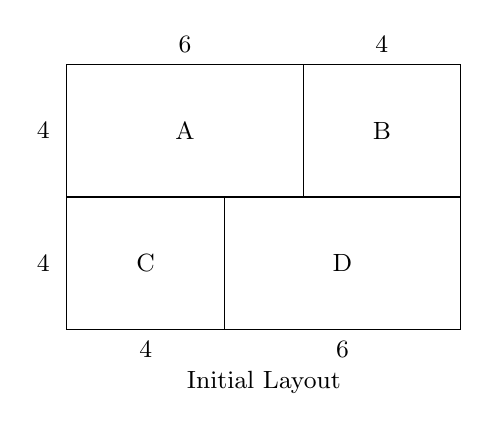
\begin{tikzpicture}[x=0.5cm,y=0.42cm,font=\small]
\draw (0,0) rectangle (10,8); \draw (0,4) -- (10,4); \draw (6,4) -- (6,8); \draw (4,0) -- (4,4);
\node at (3,6) {A}; \node at (8,6) {B}; \node at (2,2) {C}; \node at (7,2) {D};
\node at (3,8.6) {6}; \node at (8,8.6) {4}; \node at (2,-0.6) {4}; \node at (7,-0.6) {6};
\node at (-0.6,6) {4}; \node at (-0.6,2) {4};
\node at (5,-1.6) {Initial Layout};
\end{tikzpicture}\hspace{1.2cm}%
\raisebox{1.4cm}{\begin{tabular}{c|c|c|c|c|}\multicolumn{1}{c}{} & \multicolumn{1}{c}{A} & \multicolumn{1}{c}{B} & \multicolumn{1}{c}{C} & \multicolumn{1}{c}{D}\\\cline{2-5}
A & - & 1 & 1 & 3\\\cline{2-5} B & 2 & - & 2 & 1\\\cline{2-5} C & 0 & 2 & - & 2\\\cline{2-5} D & 1 & 4 & 3 & -\\\cline{2-5}\multicolumn{5}{c}{Flow Matrix}\end{tabular}}}\par\vspace{2pt}\nointerlineskip\hbox{}}{10}{L3}{CO3}
\q{2}{Illustrate and provide a summary of the typical warehouse functions and flows.}{10}{L3}{CO2}
\q{3}{State and explain the steps involved in Automated Layout Design Program (ALDEP).}{10}{L2}{CO3}
\q{4}{Explain the steps in designing of layout corresponding to typical U Flow for a manufacturing facility.}{10}{L3}{CO4}
\q{5}{With suitable assumptions propose a layout plan for setting up facilities for an information technology organization.}{10}{L4}{CO4}
\end{longtable}
\btfoot{|l|l|l|*{4}{C{0.8cm}|}*{6}{C{0.8cm}|}}{\hline
\multirow{3}{*}{Marks Distribution} & \multicolumn{2}{c|}{Particulars} & CO1 & CO2 & CO3 & CO4 & L1 & L2 & L3 & L4 & L5 & L6\\\cline{2-13}
 & Quiz & \multirow{2}{*}{Max Marks} & 10 & - & - & - & 08 & 02 & - & - & - & -\\\cline{2-2}\cline{4-13}
 & Test & & 10 & 20 & 20 & - & 10 & 30 & 10 & - & - & -\\\hline}
\stars{*******}
\end{iempaperB}

% ---------- 21IM74HD Database Management System (Improvement CIE)
\begin{iempaperB}
\paperinfo{ayear={2024-2025 (Odd Sem)},usn=0,date={19\textsuperscript{th} February 2025},code={21IM74HD},sem={VII},exam={Improvement CIE},maxmarks={10+50},duration={120},
 title={DATABASE MANAGEMENT SYSTEM},shownote=0}
\iemheadB
{\small Note: Answer all the Questions.}\par\vspace{3pt}
\begin{gtable}{Sl No}{Questions}{M}{BT}{CO}
\qpart{Part A}
\q{1.}{Identify the basic data types available for attributes in SQL.}{(02)}{L2}{CO1}
\q{2.}{Mention the guidelines for physical database design.}{(02)}{L2}{CO3}
\q{3.}{Distinguish between the base relation and virtual relation in SQL environment.}{(02)}{L3}{CO4}
\q{4.}{``Insertion, deletion and modification anomalies are considered bad in database design''. Justify.}{(02)}{L5}{CO1}
\q{5.}{Mention the expanded form of the acronym BCNF.}{(02)}{L1}{CO3}
\qpart{Part B}
\q{1}{Why is Normalization necessary while designing the relational data base? Analyze various levels in Normalization process.}{(10)}{L4}{CO1}
\q{2}{Write SQL commands to perform the following:
\begin{romi}\item[i)] To create a table student with fields: USN, SName, Address, Course, Section, TotalMarks\item[ii)] To insert values in the above table interactively\item[iii)] To create view with fields USN \& Name.\item[iv)] To change the total marks of 50 if the marks lie in between 47 \& 49.\item[v)] To delete tuples from the relation if the total marks is less than 50.\end{romi}}{(10)}{L3}{CO1}
\q{3}{Discuss insertion, deletion, and modification anomalies. Why are they considered bad? Illustrate with examples.}{(10)}{L4}{CO3}
\q{4}{Consider the following relations for an order-processing application database at ABC. Inc.\newline
ORDER (O\#, Odate, Cust\#, Total\_amount)\newline
ORDER\_ITEM(O\#, I\#, Qty\_ordered, Total\_price, Discount\%)\newline
Assume that each item has a different discount. The Total price refers to one item. Odate is the date on which the order was placed, and the Total\_amount is the amount of the order. If we apply a natural join on the relations ORDER\_ITEM and ORDER in this database, what does the resulting relation schema look like? What will be its key? Show the FDs in this resulting relation. Is it in 2NF? Is it in 3NF? Why or why not?}{(10)}{L3}{CO4}
\q{5 a}{Give an overview of different types of JOINS available in SQL.}{(06)}{L3}{CO3}
\q{b}{Distinguish between JOIN and CARTESIAN PRODUCT.}{(04)}{L4}{CO3}
\end{gtable}
\btfoot{|l|l|l|*{5}{C{0.8cm}|}*{6}{C{0.8cm}|}}{\hline
\multirow{3}{*}{\shortstack{Marks\\Distribution}} & \multicolumn{2}{c|}{Particulars} & CO1 & CO2 & CO3 & CO4 & CO5 & L1 & L2 & L3 & L4 & L5 & L6\\\cline{2-14}
 & Quiz & \multirow{2}{*}{Max Marks} & 04 & - & 4 & 2 & - & 02 & 04 & 02 & - & 02 & -\\\cline{2-2}\cline{4-14}
 & Test & & 20 & - & 20 & 10 & - & - & - & 26 & 24 & - & -\\\hline}
\stars{***}
\end{iempaperB}

% ---------- 21BT75IB Healthcare Analytics (Institutional Elective), Quiz and Test - 2 (February 2025)
\begin{iempaperB}
\paperinfo{ayear={2024-2025 (Odd Sem)},usn=0,rule=0,dept={BIOTECHNOLOGY},date={February, 2025},code={21BT75IB},sem={VII Semester},exam={Closed Book Offline Quiz and Test -- 2},maxmarks={10 + 50},duration={120 min},
 title={Healthcare Analytics (Institutional Elective)},shownote=0}
\vspace{-0.2cm}\centerline{Common to all branches}\par
\iemheadB
{\small Answer all questions in Part A \& Part B, Answer Part A in first two pages in sequence only}\par\vspace{2pt}
\begin{gtable}[Part A]{Sl No}{Questions}{M}{BT-L}{CO}
\q{1}{Write any 2 applications of systems biology.}{2}{2}{1}
\q{2}{Mass Spectrometry measures \blank[2.2cm] charge ratio (m/z) of molecules}{1}{2}{1}
\q{3}{Mention any 2 steps involved in implementation of systems biology.}{2}{2}{2}
\q{4}{List any 2 applications of secondary structure prediction.}{2}{3}{2}
\q{5}{What are the 2 gene prediction methods?}{2}{2}{3}
\q{6}{Name any tool used to detect the functional sites in a gene}{1}{4}{3}
\end{gtable}
\begin{gtable}[Part B]{Sl. No}{Questions (Test)}{M}{BT-L}{CO}
\q{1.}{Elucidate on the gene prediction methods}{10}{2}{3}
\q{2}{How does the RNA secondary be predicted?}{10}{3}{3}
\q{3}{Explain the basic structure of a protein.}{10}{4}{4}
\q{4}{Illustrate on the protein structure predictions.}{10}{4}{4}
\q{5}{Give a comprehensive note on the protein identity based on the composition.}{10}{2}{3}
\end{gtable}
\xfoot{BTL-Blooms taxonomy, CO-Course Outcomes, M-Marks}{|l|l|l|*{10}{C{0.85cm}|}}{\hline
\multirow{2}{*}{\shortstack{Marks\\Distribution}} & Particulars & & CO1 & CO2 & CO3 & CO4 & L1 & L2 & L3 & L4 & L5 & L6\\\cline{2-13}
 & Test & \shortstack{Max\\Marks} & & & 60 & 40 & & 40 & 20 & 40 & & \\\hline}
\end{iempaperB}

% ---------- 21CH751C Sustainability and Life Cycle Analysis (Institutional Elective), CIE 3
\begin{iempaperB}
\paperinfo{ayear={2024-2025 (Odd Sem)},usn=0,dept={CHEMICAL ENGINEERING},date={Feb 2025},code={21CH751C},sem={VII Semester},exam={CIE 3},maxmarks={60},duration={120 Min},
 title={SUSTAINABILITY AND LIFE CYCLE ANALYSIS (Institutional Elective)},shownote=0}
\iemheadB
{\small\bfseries Note: 1. \ Answer all the Questions.}\par\vspace{3pt}
\begin{longtable}{|C{0.9cm}|p{12.6cm}|C{0.95cm}|C{0.6cm}|C{0.6cm}|}
\hline & \multicolumn{1}{c|}{\textbf{Part A}} & M & \shortstack{B\\T} & \shortstack{C\\O}\\\hline
\illegc\ a & Define the terms odour character and odour persistence. & 2 & 1 & 2\\\hline
b & How do you control the odour arising from hydrogen sulphide? & 2 & 1 & 2\\\hline
c & Name two fermentative bacteria & 2 & 1 & 3\\\hline
d & Write a relation between intensity and concentration, & 2 & 1 & 3\\\hline
e & Name two bacteria in acetogenesis. & 2 & 1 & 2\\\hline
 & \multicolumn{1}{c|}{\textbf{Part B}} & & & \\\hline
\illegc & Explain the working of atomisers to control the odour & 10 & 2 & 3\\\hline
\illegc & State and Explain the stages of biomethanation & 10 & 2 & 4\\\hline
\illegc & With a neat sketch explain the working of fixed film digestion system & 10 & 2 & 3\\\hline
\illegc & What are the stages of bioethanol production? Explain in brief & 10 & 2 & 3\\\hline
5 & With a neat diagram explain the working of Down draft Gasifier & 10 & 2 & 4\\\hline
\end{longtable}
\par\vspace{2pt}\centerline{\small\itshape [The question numbers of Part B Q1--Q4 (left edge) are hidden by the binder ring in the scan.]}
\stars{\makebox[\textwidth]{\dotfill}}
\end{iempaperB}

% ---------- 21CM75ID Advances in Corrosion Science and Management (Improvement Test)
\begin{xpaper}
\par\vspace{2pt}\centerline{\fontsize{14}{16}\selectfont Academic year 2024-2025 (Odd Sem)}\par\vspace{2pt}
\centerline{\bfseries\fontsize{14}{16}\selectfont (IMPROVEMENT TEST FOR VII SEM)}\par\vspace{8pt}
\centerline{\bfseries DEPARTMENT OF CHEMISTRY}\par\vspace{2pt}
\noindent\begingroup\renewcommand{\arraystretch}{1.25}\fontsize{11.5}{13}\selectfont
\begin{tabular}{|C{3.6cm}|C{4.4cm}|C{4.2cm}|C{3.8cm}|}\hline
Date & 19.2.2025 & Sem - VII & Improvement test\\\hline
Course Code & 21CM75ID & Maximum Test Marks & \shortstack{Quiz-10 + Test-50\\(60M)}\\\hline
Course Name & ACSM & Duration & 120 mins\\\hline
\multicolumn{4}{|c|}{\bfseries ADVANCES IN CORROSION SCIENCE AND MANAGEMENT}\\\hline
\end{tabular}\endgroup\par\vspace{6pt}
{\bfseries Note: 1) Answer all the questions}\par
\hspace*{1.05cm}{\bfseries 2) \ Part A should be answered in the first two pages of the answer script.}\par\vspace{6pt}
\begin{longtable}{|C{1.05cm}|p{12.2cm}|C{0.95cm}|C{0.95cm}|C{0.95cm}|}
\hline & \multicolumn{1}{c|}{\textbf{Part-A}} & \textbf{M} & \textbf{BTL} & \textbf{CO}\\\hline
\q{1}{Name the type of corrosion that occurs commonly in oil and gas industries.}{1}{1}{2}
\q{2}{Arrange the following metals and alloys according to their position in the galvanic series: Gold, Aluminum, Copper, and Magnesium alloy, Bronze\newline Gold, Aluminum, Copper and Magnesium alloy, Bronze.}{1}{2}{2}
\q{3}{Suggest any one method to reduce seasonal cracking.}{1}{1}{1}
\q{4}{What is the consequence of hydrogen embrittlement?}{1}{2}{3}
\q{5}{Pitting is localized and has intense corrosion. Justify.}{1}{3}{2}
\q{6}{State any one favourable condition required for rusting to take place.}{1}{2}{1}
\q{7}{List any one disadvantage of a corrosion map.}{1}{1}{2}
\q{8}{What is the significance of the Tafel equation in corrosion studies?}{1}{3}{2}
\q{9}{How does electrical isolation help prevent differential metallic corrosion?}{1}{2}{2}
\q{10}{List any one preventive measure to avoid microbial corrosion.}{1}{1}{3}
\end{longtable}
\par\vspace{8pt}
\begin{longtable}{|C{1.05cm}|p{12.2cm}|C{0.95cm}|C{0.95cm}|C{0.95cm}|}
\hline & \multicolumn{1}{c|}{\textbf{Part-B}} & \textbf{M} & \textbf{BTL} & \textbf{CO}\\\hline
\q{11}{What are the consequences and effects of corrosion, explain with relevant examples.}{7}{2}{2}
\q{12}{What is the significance of creating a corrosion map of India, and how can it help in addressing corrosion issues more effectively?}{7}{3}{3}
\q{13}{What are the necessary steps to be taken for the corrosion test program? Explain}{7}{2}{1}
\q{14}{Two metals A and B undergo oxidation corrosion in the absence of moisture. A \illeg{}odes faster and corrosion of B takes place negligibly. Predict their Pilling-Bedworth ratio and give one example for each. Also, state the Pilling-Bedworth rule.}{7}{3}{4}
\q{15}{Differentiate between the Galvanic series and the electrochemical series, highlighting the key distinctions in their representations and significance}{7}{\illegc}{\illegc}
\q{16}{Explain the following types of corrosion\newline i) \ Crevice corrosion \ ii) Erosion corrosion}{7}{\illegc}{\illegc}
\q{17}{Enumerate four benefits and constraints associated with corrosion testing techniques.}{8}{\illegc}{\illegc}
\end{longtable}
\xfoot{BT-Blooms Taxonomy, CO-Course Outcomes, M-Marks}{|l|l|*{6}{C{0.85cm}|}l|}{\hline
\multirow{2}{*}{\shortstack{Marks\\Distribution}} & Particulars & CO1 & CO2 & CO3 & CO4 & L1 & L2 & \multirow{2}{*}{\illeg\ (cut off in the scan)}\\\cline{2-8}
 & Max Marks & 16 & 13 & 24 & 07 & 4 & 33 & \\\hline}
\stars{**********************}
\end{xpaper}

% ---------- 21CS75IE Prompt Engineering (Institutional Electives - II, Group G), Improvement CIE
\begin{iempaperB}
\paperinfo{ayear={2024-2025 (Odd \ Sem)},usn=0,dept={COMPUTER SCIENCE AND ENGINEERING},date={Feb 2025},code={21CS75IE},sem={07},exam={Improvement CIE},maxmarks={50+10},duration={120 Min},
 title={PROMPT ENGINEERING \ {\normalfont(INSTITUTIONAL ELECTVES -- II (Group G))}},shownote=0}
\iemheadB
\begin{longtable}{|C{1.05cm}|p{12.2cm}|C{0.95cm}|C{0.95cm}|C{0.95cm}|}
\hline \textbf{Q.\newline No.} & \centering\textbf{Questions}\newline\textbf{QUIZ} & \textbf{M} & \textbf{BT} & \textbf{CO}\\\hline
\qq{1.}{1.1 Role-playing prompts often begin with instructions to the model to act as a specific \blank[1.6cm] or character.}{01}{1}{1}
\qq{}{1.2 Which setting adjusts the probability distribution to control randomness in the generated text?}{01}{2}{2}
\qq{}{1.3 Why is providing context in a prompt important, and how does it help the model?}{01}{2}{2}
\qq{}{1.4 What is the significance of providing examples in prompts for complex tasks?}{01}{1}{1}
\qq{}{1.5 What is one method to prevent prompt injection in AI models?}{01}{1}{1}
\qq{}{1.6 How does prompt leaking impact AI security?}{01}{1}{1}
\qq{}{1.7 Name one strategy to prevent AI jailbreaking.}{01}{1}{2}
\qq{}{1.8 Why is human feedback important in reinforcement learning?}{01}{2}{3}
\qq{}{1.9 What role does reward function play in reinforcement learning?}{01}{1}{1}
\q{}{1.10 \ Name one key algorithm used in reinforcement learning for planning.}{01}{1}{1}
\q{}{\centering TEST}{}{}{}
\qq{2.}{(a)Describe an example where PAL can enhance the performance of a language model.}{05}{2}{3}
\q{}{(b)Explain the concept of chain-of-thought (CoT) prompting and its significance in reasoning tasks.}{05}{1}{2}
\q{3}{Classify and explain the types of Large Language Model (LLM) prompts based on the type of information being prompted. Provide examples for each type.}{10}{1}{2}
\q{4}{What is multimodal prompting in AI models? Discuss its significance and challenges in integrating different types of data (text, images, audio, etc.).}{10}{1}{2}
\q{5}{Define graph prompting and discuss its role in enhancing reasoning capabilities \illeg\ language models.}{\illegc}{\illegc}{\illegc}
\q{6}{How can adversarial attacks such as prompt injection and jailbreaking impact \illeg\ security of AI systems? Suggest possible mitigation strategies.}{\illegc}{\illegc}{\illegc}
\end{longtable}
\stars{***********}
\xfoot{BT-Blooms Taxonomy, CO-Course Outcomes}{|l|l|l|*{8}{C{0.85cm}|}l|}{\hline
\multirow{2}{*}{\shortstack{Marks\\Distribution}} & \multicolumn{2}{c|}{Particulars} & CO1 & CO2 & CO3 & CO4 & CO5 & L1 & L2 & L3 & \multirow{2}{*}{\illeg\ (cut off)}\\\cline{2-11}
 & \shortstack{Test \&\\Quiz} & \shortstack{Max\\Marks} & 06 & 28 & 16 & 00 & 10 & 32 & 18 & 00 & \\\hline}
\cotable{Course Outcomes:}{CO1: & Demonstrate an understanding of prompt engineering principles including how \illeg\ structure and phrasing impact the performance of AI models.\\\hline
CO2: & Design and implement effective prompts- to create and apply prompts for various \illeg\ language processing (NLP) tasks, such as text generation, summarization, and \illeg\ AI models.\\\hline
CO3: & Critically evaluate the effectiveness of prompts - assess the quality and performance \illeg\ in terms of accuracy, coherence, and relevance, identifying areas for improvement.\\\hline
CO4: & Apply prompt engineering techniques in real-world scenarios - use prompt engineering \illeg\ strategies to address practical problems in domains such as education, healthcare, and \illeg\ demonstrating the applicability of AI-driven solutions.\\\hline
CO5: & Collaborate on projects involving prompt engineering - work effectively in teams to \illeg\ implement, and evaluate prompt-based solutions, showcasing their ability to contribute \illeg\ complex AI-related projects.}
\end{iempaperB}

% ---------- 21CV75IF Integrated Health Monitoring of Structures (Improvement CIE)
\begin{xpaper}
\par\vspace{2pt}\centerline{\sansfont\fontsize{12}{14}\selectfont Department of Civil Engineering}\par\vspace{8pt}
\ofour{19-02-2025}{50+10}{\textbf{21CV75IF}}{120 Min}{VII}{IMPROVEMENT CIE}{INTEGRATED HEALTH MONITORING OF STRUCTURES}
{\small Note: Answer all questions.}\par\vspace{3pt}
\begin{gtable}[QUIZ]{Sl.\newline No.}{Questions}{M}{BT}{CO}
\q{1}{Sensors measure physical parameters such as \blank[1.4cm], \blank[1.4cm], \blank[1.4cm] during testing. (any 2)}{2}{1}{2}
\q{2}{Two main types of Dynamic Analysis are \blank[1.6cm] and \blank[1.6cm]}{2}{1}{4}
\q{3}{List any two characteristics of Static Response Measurement}{2}{1}{3}
\q{4}{Mention any two advantages of Dynamic Response methods.}{2}{1}{4}
\q{5}{List the different NDT methods (any 4)}{2}{1}{4}
\end{gtable}
\begin{gtable}[TEST]{Sl.\newline No.}{Questions}{M}{BT}{CO}
\q{1}{Explain the objectives of Static response systems and Discuss the measurement techniques used for static response systems..}{10}{2}{3}
\q{2}{List and discuss the different types of Dynamic Response Methods}{10}{2}{3}
\q{3}{Discuss different remote SHM techniques, systems and challenges}{10}{2}{4}
\q{4}{Describe remote data acquisition systems and discuss the components used}{10}{3}{4}
\q{5}{Explain different Simulation methods and loading methods of Static Field Testing.}{10}{3}{3}
\end{gtable}
{\small\bfseries Course outcomes:}\par
\btfoot{|l|l|l|*{10}{C{0.8cm}|}}{\hline
\multirow{2}{*}{\shortstack{Marks\\Distribution}} & \multicolumn{2}{c|}{Particulars} & CO1 & CO2 & CO3 & CO4 & L1 & L2 & L3 & L4 & L5 & L6\\\cline{2-13}
 & Test & Max Marks & - & 2 & 32 & 26 & 10 & 30 & 20 & & & \\\hline}
\stars{***********}
\end{xpaper}

% ---------- 21EE75IH E-Mobility (Test - III)
\begin{xpaper}
\par\vspace{2pt}\centerline{\sansfont\fontsize{12}{14}\selectfont Department of Electrical \& Electronics Engineering}\par\vspace{8pt}
\centerline{\fontsize{14}{16}\selectfont Academic Year 2024-25 (ODD SEM)}\par\vspace{8pt}
\ofour{19\textsuperscript{th} Feb 2024}{50}{21EE75IH}{90 Mins}{VII Semester}{TEST-III}{E-Mobility}
\begin{longtable}{|C{1.05cm}|p{11.6cm}|C{1.3cm}|C{0.95cm}|C{0.95cm}|}
\hline \textbf{Q.No} & \multicolumn{1}{c|}{\textbf{Part B -- Test Questions}} & \textbf{Marks} & \textbf{COs} & \textbf{BT}\\\hline
\q{1a.}{Draw and explain the functions of components involved in Low power charger}{06}{4}{2}
\q{1b.}{Mention voltage and current levels of AC and DC charging.}{04}{2}{1}
\q{2.}{With the neat sketch of circuit diagram and waveforms explain the operation of Boost Converter for Power Factor Correction.}{\corr{06}{10}}{4}{3}
\q{3a.}{Write the various EV charging standards and discuss briefly about \textbf{\textit{SAE J1772.}}}{05}{2}{2}
\q{3b.}{Discuss briefly about wireless charging of electric vehicle.}{05}{2}{2}
\q{4.}{Discuss the following with respect considerations for sizing of drive system.\newline
{\small (a) Sizing the propulsion motor\newline (b) Matching the electric machine and the internal combustion engine (ICE).}}{10}{4}{2}
\q{5a.}{Discuss briefly about typical CAN layout in electric vehicle.}{05}{3}{3}
\q{5b.}{Explain about CAN message frame.}{05}{3}{3}
\end{longtable}
\btfoot{|l|l|l|*{10}{C{0.85cm}|}}{\hline
\multirow{2}{*}{\shortstack{Marks\\Distribution}} & \multicolumn{2}{c|}{Particulars} & CO1 & CO2 & CO3 & CO4 & L1 & L2 & L3 & L4 & L5 & L6\\\cline{2-13}
 & Test & \shortstack{Max\\Marks} & - & 14 & 10 & 26 & 4 & 26 & 16 & - & - & -\\\hline}
\stars{***********}
\par\centerline{\scriptsize\itshape (The struck-out mark for Q2 was corrected by hand on the original.)}
\end{xpaper}

% ---------- 21EE75IH E-Mobility (Quiz - III)
\begin{xpaper}
\par\vspace{2pt}\centerline{\sansfont\fontsize{12}{14}\selectfont Department of Electrical \& Electronics Engineering}\par\vspace{8pt}
\centerline{\fontsize{14}{16}\selectfont Academic Year 2024-25 (ODD SEM)}\par\vspace{8pt}
\ofour{19\textsuperscript{th} Feb 2024}{\illeg}{21EE75IH}{\illeg}{VII Semester}{QUIZ-III}{E-Mobility}
\begin{longtable}{|C{1.05cm}|p{11.6cm}|C{1.3cm}|C{0.95cm}|C{0.95cm}|}
\hline \textbf{Q.No.} & \multicolumn{1}{c|}{\textbf{Part A -- Quiz Questions}} & \textbf{Marks} & \textbf{COs} & \textbf{BT}\\\hline
\q{1.}{What are the key requirements of an EV charging system?}{02}{2}{\illegc}
\q{2.}{Why is power factor correction important in battery charging?}{02}{2}{\illegc}
\q{3.}{What is the function of an AC-DC converter in an EV charger?}{02}{2}{\illegc}
\q{4.}{What is the role of a communication protocol in EV charging?}{02}{3}{\illegc}
\q{5.}{What role does an onboard charger play in an EV?}{02}{3}{\illegc}
\end{longtable}
\btfoot{|l|l|l|*{10}{C{0.85cm}|}}{\hline
\multirow{2}{*}{\shortstack{Marks\\Distribution}} & \multicolumn{2}{c|}{Particulars} & CO1 & CO2 & CO3 & CO4 & L1 & L2 & L3 & L4 & L5 & L6\\\cline{2-13}
 & Test & \shortstack{Max\\Marks} & - & 06 & 04 & - & 06 & 03 & 01 & - & \illegc & \illegc\\\hline}
\stars{***********}
\end{xpaper}

% ---------- 21ET75IK Space Technology and Applications (CIE-III)
\begin{xpaper}
\par\vspace{2pt}\centerline{\sansfont\fontsize{12}{14}\selectfont Department of Electronics \& Telecommunication Engineering}\par\vspace{6pt}
\noindent\begingroup\renewcommand{\arraystretch}{1.3}\fontsize{11.5}{13}\selectfont
\begin{tabular}{|C{3.6cm}|p{4.6cm}|C{4.0cm}|C{3.8cm}|}\hline
Date & 19\textsuperscript{th} FEB. 2025 & \shortstack{Maximum\\Marks/Quiz} & 50+10\\\hline
Course Code/Title & 21ET75IK & Duration & 120 Min\\\hline
Sem & VII Semester & \multicolumn{2}{c|}{CIE-III}\\\hline
\multicolumn{4}{|c|}{\bfseries\fontsize{13}{15}\selectfont SPACE TECHNOLOGY AND APPLICATIONS}\\\hline
\end{tabular}\endgroup\par\vspace{6pt}
\begin{gtable}{Q.No}{PART A}{M}{BT}{CO}
\q{1.}{Define Multispectral Image.}{1}{L1}{CO3}
\q{2.}{What is Spatial and Spectral resolution?}{1}{L2}{CO3}
\q{3.}{Mention few applications of Remote sensing}{1}{L1}{CO4}
\q{4.}{Who was the first person to walk on the moon?}{1}{L1}{CO4}
\q{5.}{Define Space debris.}{1}{L1}{CO4}
\q{6.}{What is the difference between space shuttle and spacecraft?}{1}{L2}{CO4}
\q{7.}{Differentiate between the US Apollo Mission and the India Chandrayaan -1 mission?}{2}{L2}{CO4}
\q{8.}{What are the most common applications of satellite in day to day life? Mention any four.}{2}{L2}{CO1}
\qpart{PART B}
\q{1.}{Explain how image processing and analysis applied in remote sensing. Illustrate relevant techniques used.}{10}{L2}{CO3}
\q{2.}{Explain different types of remote sensing cameras by mentioning their various characteristics and differences.}{10}{L2}{CO3}
\q{3.}{Describe at least two remote sensing satellites launched by India and highlight their applications.}{10}{L2}{CO4}
\q{4.a)}{What are the Procedures adopted for Disaster and flood management system and explain with the help of a neat diagram.}{05}{L2}{C3}
\q{b)}{Write a short note on ``Inter space communication system''}{05}{L2}{C3}
\q{5.}{Give explanatory notes on:\newline
\hspace*{0.4cm}i) \ Planetary Payloads\newline \hspace*{0.4cm}ii) Zero gravity experiments.}{10}{L2}{CO4}
\end{gtable}
\btfoot{|l|l|l|*{10}{C{0.85cm}|}}{\hline
\multirow{2}{*}{\shortstack{Marks\\Distribution}} & \multicolumn{2}{c|}{Particulars} & CO1 & CO2 & CO3 & CO4 & L1 & L2 & L3 & L4 & L5 & L6\\\cline{2-13}
 & Test & \shortstack{Max\\Marks} & 01 & --- & 32 & 17 & 06 & 44 & -- & -- & -- & --\\\hline}
\end{xpaper}

% ---------- 21IM75IM Project Management (Improvement Test)
\begin{iempaperB}
\paperinfo{ayear={2024-2025 (ODD Sem)},usn=0,date={19 FEB 2025},code={21IM75IM},sem={VII},exam={Improvement Test},maxmarks={65},duration={120 Min},
 title={PROJECT MANAGEMENT},shownote=0}
\iemheadB
\onenote{Answer all the Questions.}
\begin{gtable}[PART -- A]{Sl.\newline No.}{Questions}{M}{BT}{CO}
\q{1}{Which costs are included in project life cycle costing?}{02}{L2}{CO1}
\q{2}{What are the four main stages of Product Lifecycle Management (PLM)?}{02}{L2}{CO1}
\q{3}{What is resource levelling in project scheduling?}{02}{L2}{CO2}
\q{4}{What are the two major network-based scheduling techniques?}{02}{L2}{CO1}
\q{5}{What is project implementation scheduling?}{02}{L2}{CO2}
\end{gtable}
\begin{gtable}[PART -- B]{Sl.\newline No.}{Questions}{M}{BT}{CO}
\q{1.}{A manufacturing company is launching a new product and needs to plan its project schedule efficiently. As a project manager, explain the steps involved in project implementation scheduling and discuss how effective time management and resource allocation methods can optimize the project timeline.}{10}{L3}{CO3}
\q{2.}{A construction company is implementing a new infrastructure project. How can different scheduling techniques and PLM (Product Lifecycle Management) concepts be used to optimize project planning? Additionally, explain the significance of life cycle costing in project management.}{10}{L3}{CO3}
\q{3.}{A project consists of the following activities with their estimated durations (in days) and dependencies:
\qtabc{|c|c|c|}{\hline \textbf{Activity} & \textbf{Predecessor(s)} & \textbf{\shortstack{Duration\\(Days)}}\\\hline A & - & 5\\\hline B & A & 4\\\hline C & A & 6\\\hline D & B & 3\\\hline E & B, C & 7\\\hline F & D, E. & 5\\\hline}
\textbf{Tasks:}
\begin{num}\item Construct the Project Network Diagram.\item Identify the Earliest Start Time (ES), Earliest Finish Time (EF), Latest Start Time (LS), and Latest Finish Time (LF) for each activity.\item Determine the critical path and the total project duration.\end{num}}{15}{L4}{CO4}
\q{4.}{A project consists of the following activities with their estimated time durations in weeks:
\qtabc{|c|c|c|c|c|}{\hline \textbf{Activity} & \textbf{Predecessor} & \textbf{\shortstack{Optimistic\\(a)}} & \textbf{\shortstack{Most Likely\\(m)}} & \textbf{\shortstack{Pessimistic\\(b)}}\\\hline A & - & 2 & 4 & 6\\\hline B & A & 3 & 6 & 9\\\hline C & A & 4 & 5 & 6\\\hline D & B & 2 & 3 & 8\\\hline E & C & 3 & 4 & 5\\\hline F & D,E & 4 & 6 & 8\\\hline}
\textbf{Tasks:}
\begin{num}\item Construct the Project Network Diagram.\item Compute the Expected Time (TE) for each activity\item Identify the Critical Path and the Project Completion Time.\end{num}}{\illegc}{\illegc}{\illegc}
\end{gtable}
\btfoot{|l|l|l|*{5}{C{0.8cm}|}*{3}{C{0.8cm}|}l|}{\hline
\multirow{3}{*}{\shortstack{Marks\\Distribution}} & \multicolumn{2}{c|}{Particulars} & CO1 & CO2 & CO3 & CO4 & CO5 & L1 & L2 & L3 & \multirow{3}{*}{\illeg\ (cut off)}\\\cline{2-11}
 & \multirow{2}{*}{\shortstack{Max\\Marks}} & Quiz & 6 & 4 & & & & & 10 & & \\\cline{3-11}
 & & Test & & & 20 & 30 & & & & 20 & \\\hline}
\stars{*****}
\end{iempaperB}

% ---------- 21ME75IO (as printed) Nuclear Engineering, CIE-III (Improvement Quiz and Test)
\begin{iempaperB}
\paperinfo{ayear={2024-2025 (ODD Sem)},dept={MECHANICAL ENGINEERING},date={19/02/2025},code={21ME75IO},sem={VII},exam={CIE-III (Improvement Quiz and Test)},maxmarks={10 (Q) + 50 (T)},duration={120 Min.},
 title={NUCLEAR ENGINEERING},shownote=0}
\iemheadB
{\small Answer all the Questions.}\par\vspace{3pt}
\begin{gtable}{\#}{Questions}{M}{BT}{CO}
\qpart{Part -- A (Quiz)}
\q{1}{A nuclear unit becoming critical means \ldots\ldots\ldots\ldots}{01}{L1}{01}
\q{2}{Moderator in nuclear plants is used to \ldots\ldots\ldots\ldots}{01}{L1}{01}
\q{3}{The most commonly used moderator in nuclear plants is \ldots\ldots\ldots\ldots}{01}{L1}{01}
\q{4}{Breeder reactor has a conversion ratio of \ldots\ldots\ldots\ldots}{01}{L2}{01}
\q{5}{One gram of uranium will produce energy equivalent to approximately \ldots\ldots\ldots tonne of high-grade coal.}{01}{L2}{01}
\q{6}{The commonly used material for shielding is \ldots\ldots\ldots\ldots}{01}{L1}{01}
\q{7}{The main interest of shielding in nuclear reactor is protection against \ldots\ldots\ldots\ldots}{01}{L1}{01}
\q{8}{Reflector in nuclear plants is used to \ldots\ldots\ldots\ldots}{01}{L1}{01}
\q{9}{The energy required to be applied to a radioactive nucleus for the emission of a neutron is\ldots.}{01}{L2}{01}
\q{10}{Enriched uranium is one in which \ldots\ldots\ldots\ldots}{01}{L2}{01}
\qpart{Part -- B}
\q{1}{Explain with a sketch the elements of a nuclear reactor.}{10}{L3}{02}
\q{2}{Explain the factors that control the site selection of nuclear power plant.}{10}{L4}{02}
\q{3}{Give the classification of nuclear reactors using various parameters.}{10}{L5}{03}
\q{4}{A 230 g piece of boron (mol wt. 10) absorbs thermal neutrons at the rate of 9.57 x 10\textsuperscript{13} per (cm\textsuperscript{3} s). Boron density is 2.3 g/cm\textsuperscript{3}. Find (a) the thermal neutron flux, and (b) the average distance that a neutron travels before it is absorbed. For thermal neutrons, $\sigma_a$ = 755 barns and $\sigma_s$ = 4.0 barns.}{10}{L5}{03}
\q{5}{A reactor is fuelled with 100 tonnes of natural uranium (atomic mass 238.05) in which the average thermal neutron (2200 m/s) flux is 10\textsuperscript{13} neutrons/cm\textsuperscript{2}s, The 2200 m/s cross section of U-235 (atomic mass 235.04) are: $\sigma_f$ = 579 barns and $\sigma_c$ = 101 barns. The energy release per fission is 200 MeV and 0.715\% of natural uranium is U-235. Calculate (a) the rating of the reactor in MW/tonne, (b) the rate of consumption of U-235 per day.}{10}{L6}{04}
\end{gtable}
\btfoot{|l|l|*{10}{C{0.85cm}|}}{\hline
\multirow{2}{*}{\shortstack{Marks\\Distribution}} & Particulars & CO1 & CO2 & CO3 & CO4 & L1 & L2 & L3 & L4 & L5 & L6\\\cline{2-12}
 & MaxMarks & 10 & 20 & 20 & 10 & 06 & 04 & 10 & 10 & 20 & 10\\\hline}
\stars{*****All The Best*****}
\end{iempaperB}

% ---------- 21HS75IQ Cognitive Psychology (CIE-III, Improvement Test)
\begin{iempaperB}
\paperinfo{ayear={2024-2025 (ODD Sem)},usn=0,dept={Humanities and Social Sciences},date={19\textsuperscript{th} February 2025},code={21HS75IQ},sem={VII},exam={CIE -- III- Improvement Test},maxmarks={10 + 50},duration={30 + 90 Min},
 title={Cognitive Psychology},shownote=0}
\iemheadB
{\small Note: Answer all the Questions.}\par\vspace{3pt}
\begin{longtable}{|C{1.05cm}|p{12.2cm}|C{0.95cm}|C{0.95cm}|C{0.95cm}|}
\hline & \multicolumn{1}{l|}{\textbf{Part -- A- Quiz}} & \multicolumn{3}{c|}{\textbf{10 Marks}}\\
\textbf{Sl. No.} & \textbf{Questions} & \textbf{M} & \textbf{BT} & \textbf{CO}\\\hline
\q{1.1}{What properties characterize language?}{2}{L1}{CO1}
\q{1.2}{What is the difference between phonemes and morphemes?}{2}{L1}{CO1}
\q{1.3}{Which processes can be impaired in dyslexia?}{2}{L1}{CO2}
\q{1.4}{What are the fundamental structures and processes within the brain?}{2}{L2}{CO2}
\q{1.5}{Why is the study of brain disorders useful for cognitive psychologists?}{2}{L2}{CO2}
& \multicolumn{1}{l|}{\textbf{Part -- B}} & \multicolumn{3}{c|}{\textbf{50 Marks}}\\
Q. No & Questions & \textbf{M} & \textbf{BT} & \textbf{CO}\\\hline
\q{2}{Compare and contrast the kinds of understandings that can be gained by studying speech errors made by healthy people with those that can be gained by studying the language produced by people who have particular brain lesions.}{10}{L1}{CO1}
\q{3}{Explain in detail how cognitive psychologists should interpret evidence of linguistic universals when considering the linguistic-relativity hypothesis.}{10}{L2}{CO2}
\q{4}{Researchers already are aware that a deficit of a neurotransmitter, acetylcholine, in the hippocampus is linked to Alzheimer's disease. Given the difficulty of reaching the hippocampus without causing other kinds of brain damage, how might researchers try to treat Alzheimer's disease?}{10}{L3}{CO2}
\q{5}{What is an area of cognition that could be studied effectively by viewing the structure or function of the human brain? Describe how a researcher might use one of the techniques to study that area of cognition.}{10}{L1}{CO1}
\q{6}{Explain some of the reasons that researchers are interested in finding out the localization of function in the human brain.}{10}{L2}{CO2}
\end{longtable}
\btfoot{|l|l|l|*{10}{C{0.8cm}|}}{\hline
\multirow{2}{*}{\shortstack{Marks\\Distribution}} & \multicolumn{2}{c|}{Particulars} & CO1 & CO2 & CO3 & CO4 & L1 & L2 & L3 & L4 & L5 & L6\\\cline{2-13}
 & Test & Max Marks & 10 & 20 & 20 & -- & 20 & 20 & 10 & -- & -- & --\\\hline}
\end{iempaperB}

% ---------- 21HS75IR Principles & Practices of Cyber Law (Improvement Test)
\begin{iempaperB}
\paperinfo{ayear={2024-2025 (ODD SEM)},usn=0,dept={INDUSTRIAL ENGINEERING\& MANAGEMENT},date={19/02/2025},code={21HS75IR},sem={VII},exam={IMPROVEMENT TEST},maxmarks={10+50},duration={120 Mins},
 title={PRINCIPLES \& PRACTICES OF CYBER LAW},shownote=0}
\iemheadB
{\small Note: Answer all the Questions.}\par\vspace{3pt}
\begin{longtable}{|C{1.05cm}|p{12.2cm}|C{0.95cm}|C{0.95cm}|C{0.95cm}|}
\hline Q.No. & \multicolumn{1}{c|}{\textbf{PART- A}} & M & BT & CO\\\hline
\q{1}{Name the two different types of data with their meaning}{2}{3}{CO2}
\q{2}{Define Meta-Data.}{2}{2}{CO3}
\q{3}{What are Forensic Tools ?}{2}{2}{CO2}
\q{4}{What is an FIR in the context of Cyber Crime Investigation?}{2}{2}{CO2}
\q{5}{What is a Charge Sheet in Cyber Crime Investigation?}{2}{2}{CO2}
\qpart{PART -B}
\q{1}{Define Cyber Crime Cells (CCCs) and discuss their role in the investigation of cybercrimes.}{10}{02}{CO3}
\q{2}{Explain the structure and key functions of Cyber Crime Cells in India.}{10}{02}{CO3}
\q{3}{Explain the process of cyber crime investigation in detail, including the role of law enforcement agencies, evidence collection, and legal procedures.}{10}{03}{CO3}
\q{4}{Discuss the need to protect data in cyberspace and the types of data that require protection.}{10}{03}{CO2}
\q{5a}{Discuss the General Data Protection Regulations (GDPR) 2016.}{05}{03}{CO2}
\q{5b}{How can organizations ensure compliance with data protection regulations?}{05}{03}{CO2}
\end{longtable}
\btfoot{|l|l|l|*{10}{C{0.8cm}|}}{\hline
\multirow{2}{*}{Marks Distribution} & \multicolumn{2}{c|}{Particulars} & CO1 & CO2 & CO3 & CO4 & L1 & L2 & L3 & L4 & L5 & L6\\\cline{2-13}
 & Test & Max Marks & - & 28 & 32 & - & - & 18 & 42 & - & - & -\\\hline}
\stars{******}
\end{iempaperB}

% (scan p25 is a blurred duplicate of the 21HS71 CIE-II paper of 27 Jan 2025, typeset from a clear copy in s7-cie2a.tex)

\end{document}
